\begin{figure}[H]
	\begin{center}
	\begin{tabular}[c]{c c}
		\begin{tabular}[c]{c c c c}
			
\includegraphics[scale=.1125]{m0_reg.png} &
			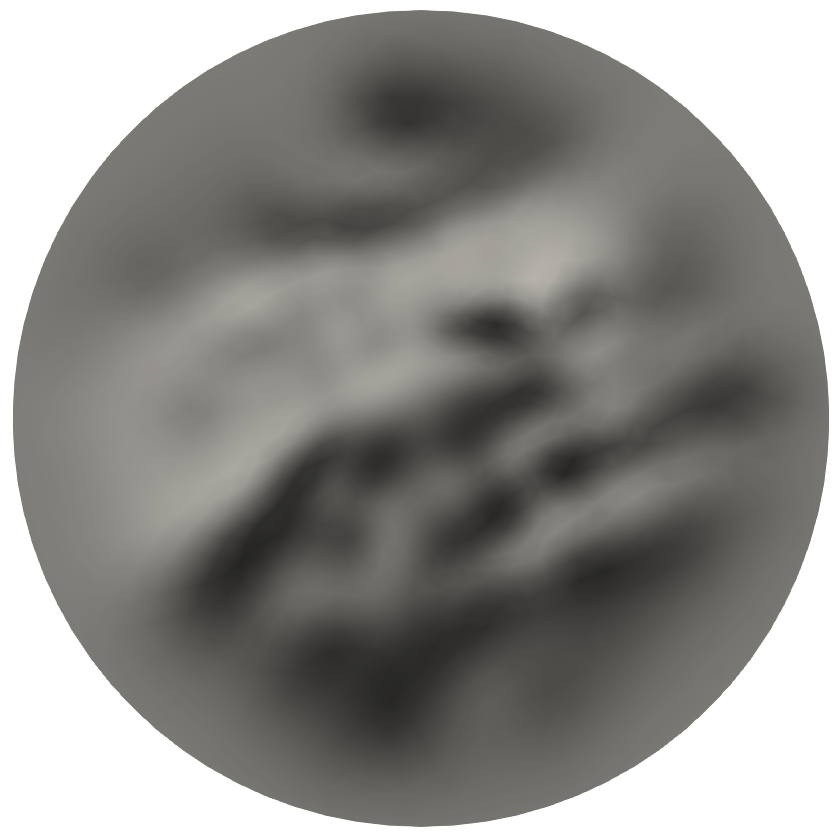
\includegraphics[scale=.1125]{m3_reg.png} &
			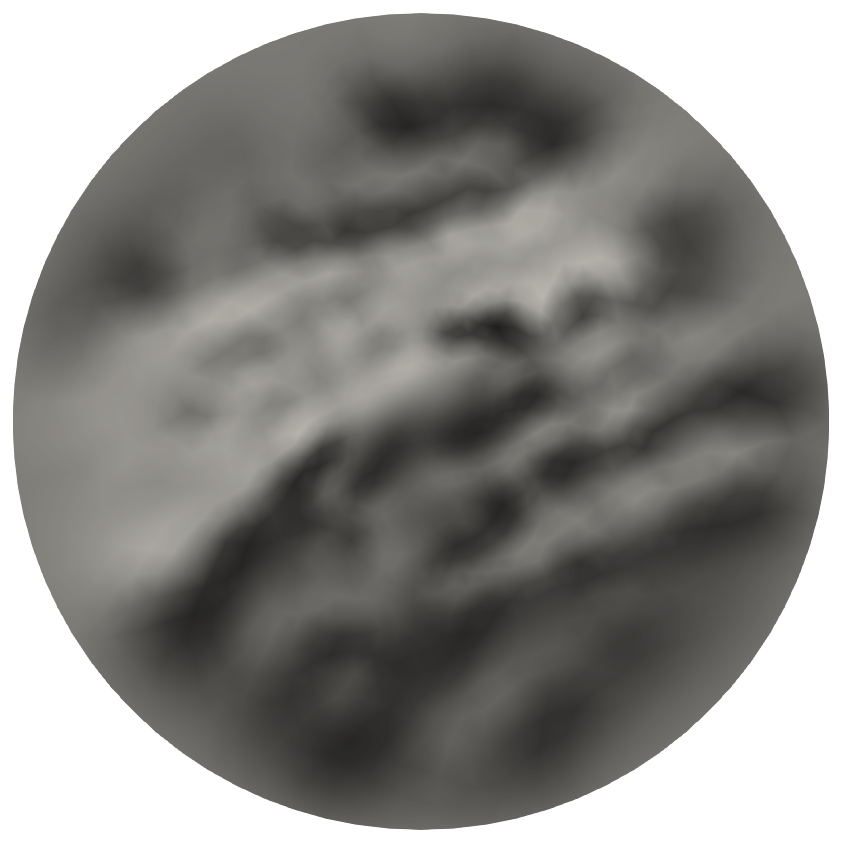
\includegraphics[scale=.1125]{m4_reg.png} &
			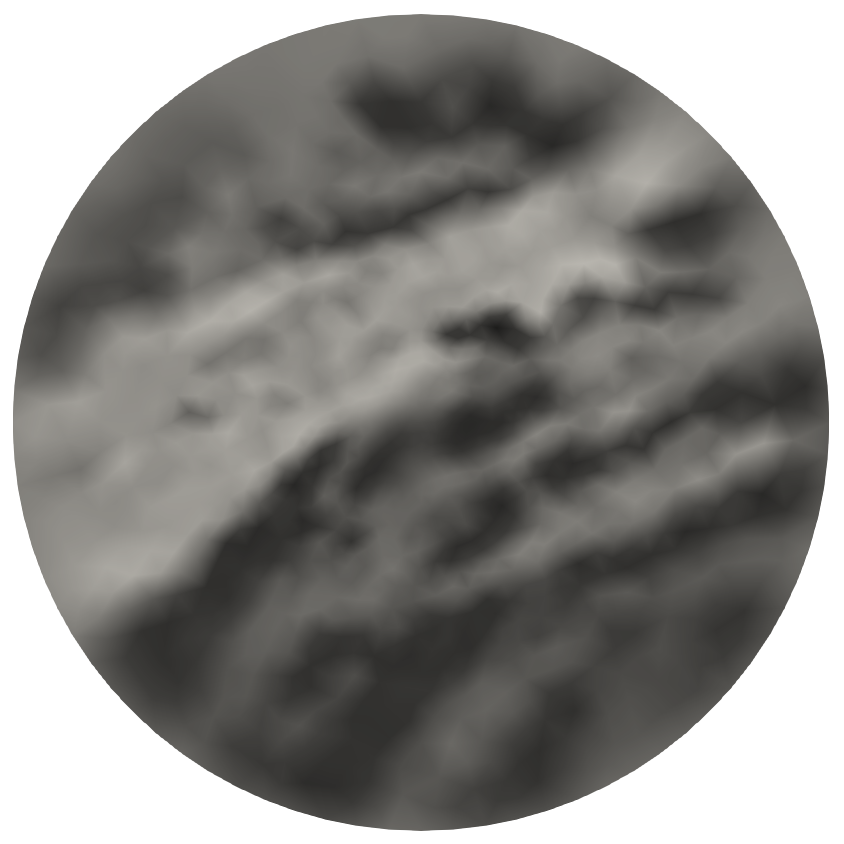
\includegraphics[scale=.1125]{m5_reg.png} \\
			
\includegraphics[scale=.1125]{m0_none.png} &
			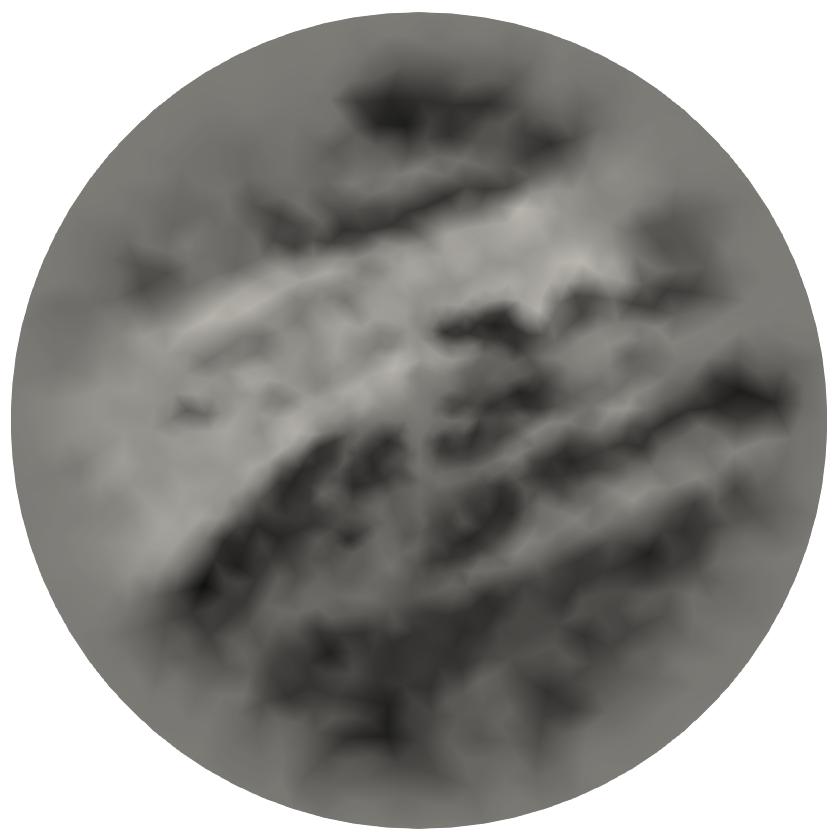
\includegraphics[scale=.1125]{m3_none.png} &
			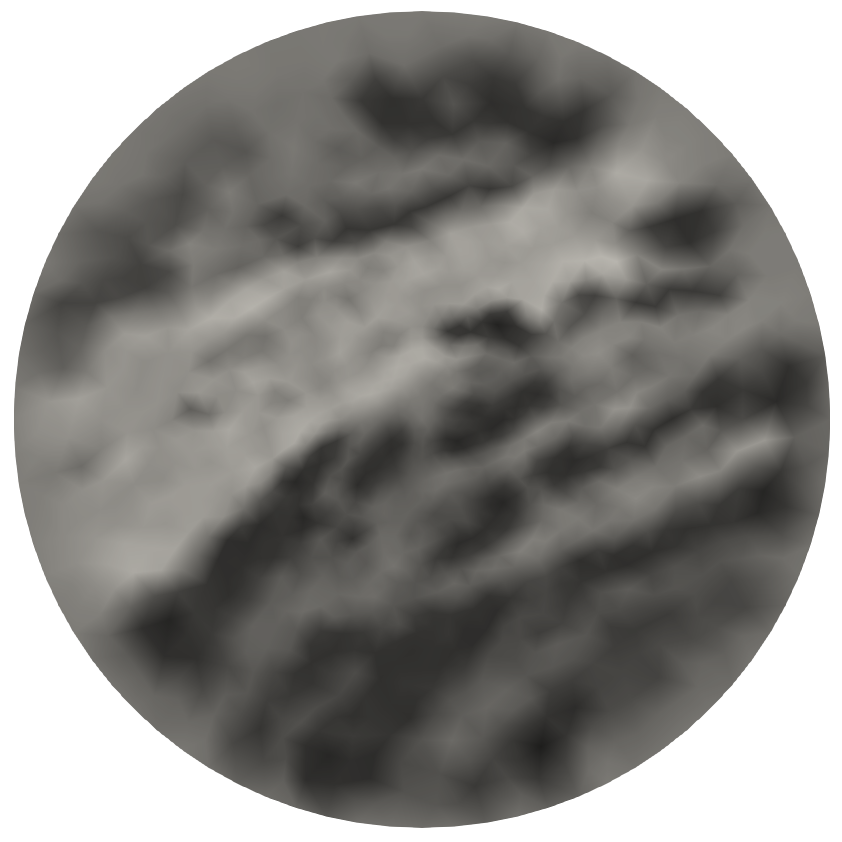
\includegraphics[scale=.1125]{m4_none.png} &
			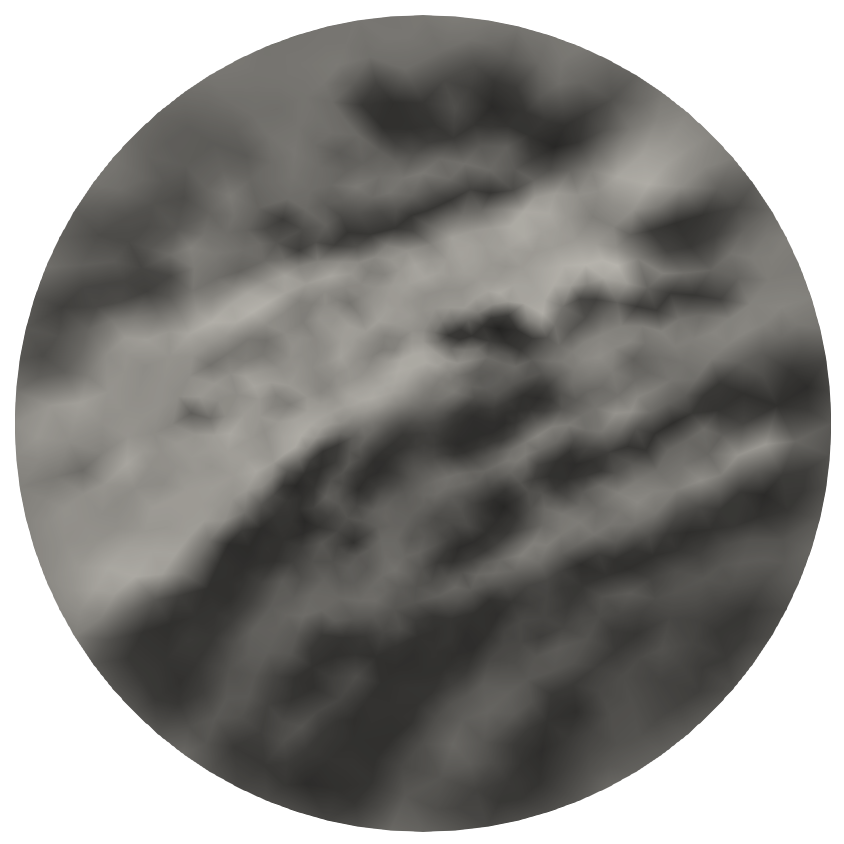
\includegraphics[scale=.1125]{m5_none.png} \\
			
\includegraphics[scale=.1125]{m0_psf.png} &
			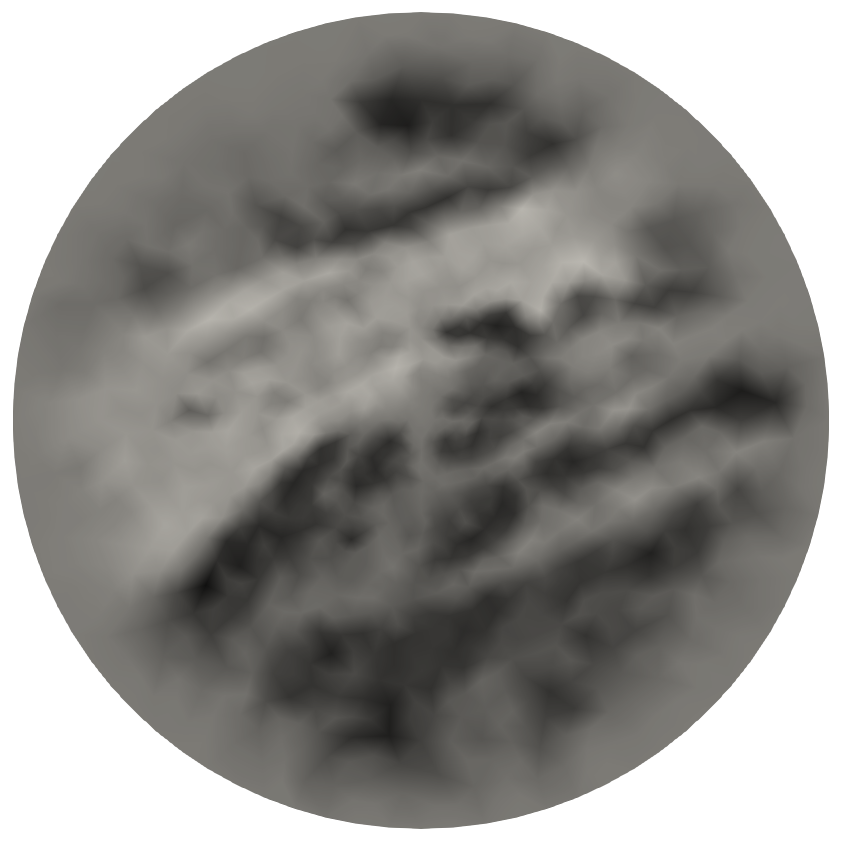
\includegraphics[scale=.1125]{m3_psf.png} &
			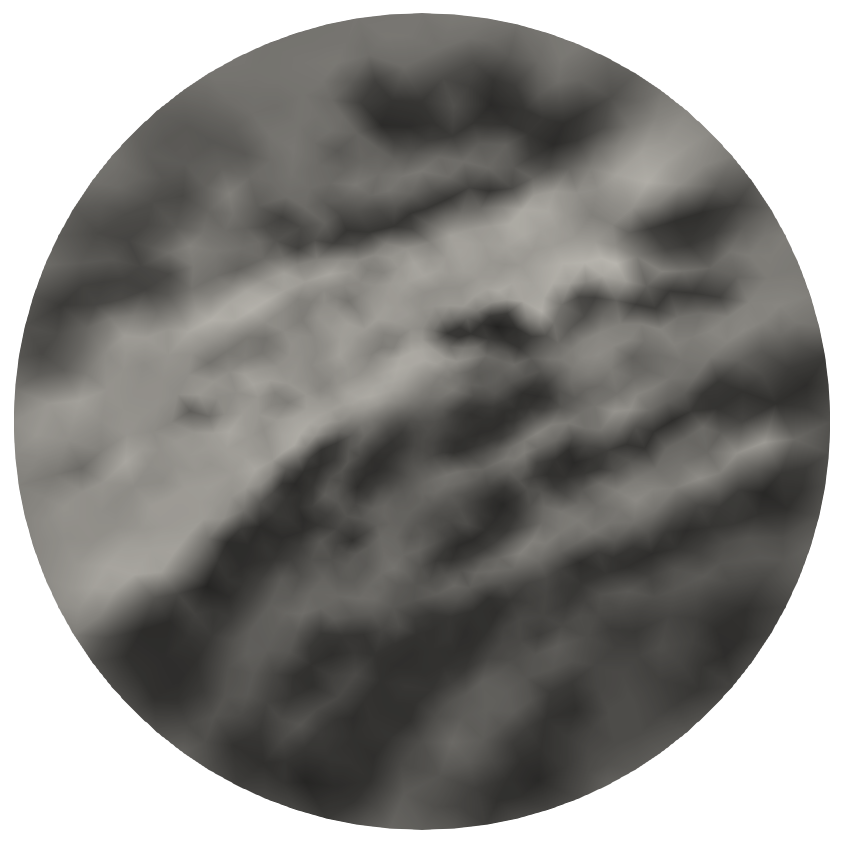
\includegraphics[scale=.1125]{m4_psf.png} &
			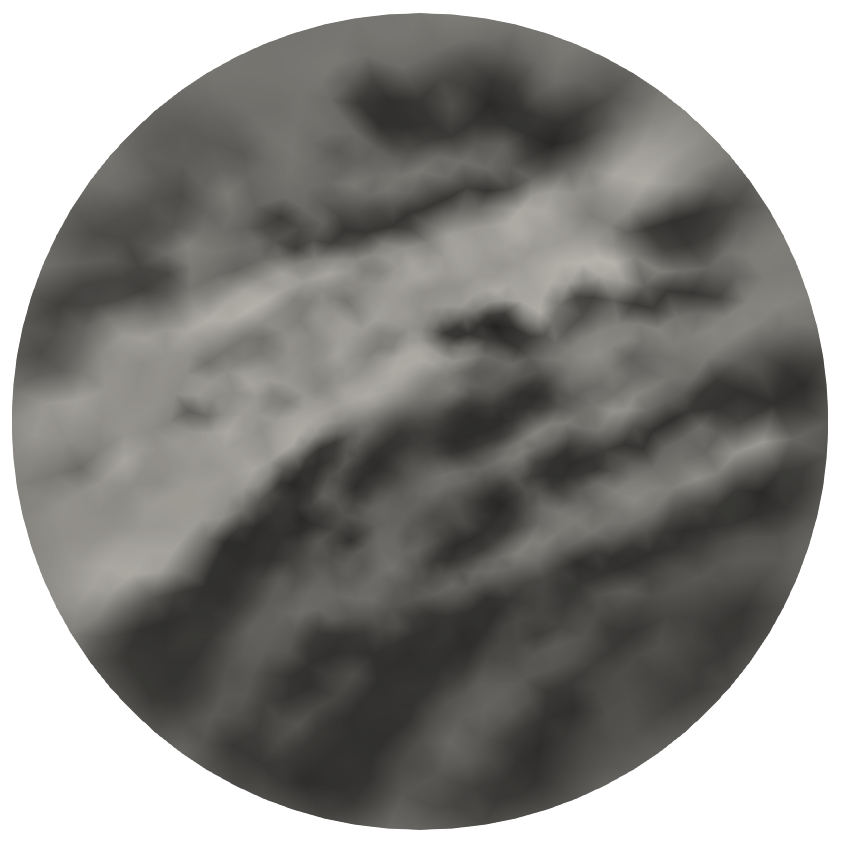
\includegraphics[scale=.1125]{m5_psf.png} 
		\end{tabular} 
		&
		\begin{tabular}[c]{c}
		 \\
		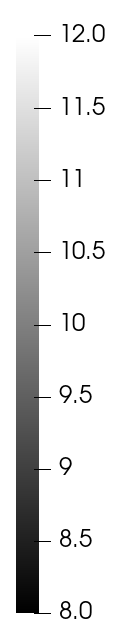
\includegraphics[scale=.25]{mColorBar.png} \\
		\end{tabular}
	\end{tabular}
	\caption{The initial parameter (left column), the parameter after three (second column)- four (third column) and five (right column) Newton iteration, the parameter after four Newton iterations for regularization preconditioning (upper row), no preconditioning (middle row) and psf preconditioning (lower row).}
	\end{center}
\end{figure}
